%Packages
\documentclass[12pt, a4paper]{article}
\usepackage[top=2cm, bottom=3cm, left=2cm, right=2cm]{geometry}
\usepackage{amsmath,amsthm,amsfonts,amssymb,amscd, fancyhdr, color, comment, graphicx, environ}
\usepackage{float}
\usepackage{lastpage}
\usepackage[dvipsnames]{xcolor}
\usepackage[framemethod=TikZ]{mdframed}
\usepackage{enumerate}
\usepackage[shortlabels]{enumitem}
\usepackage{fancyhdr}
\usepackage{indentfirst}
\usepackage{listings}
\usepackage{sectsty}
\usepackage{thmtools}
\usepackage{shadethm}
\usepackage{hyperref}
\usepackage{setspace}
\usepackage[section]{placeins}

\hypersetup{
    colorlinks=true,
    linkcolor=blue,
    filecolor=magenta,      
    urlcolor=blue,
}
\usepackage{xcolor}
\usepackage{amsfonts,amssymb}
\usepackage[ruled,vlined]{algorithm2e}
\usepackage{amsmath}

%New colors defined below
\definecolor{codegreen}{rgb}{0.22,0.49,0.13}
\definecolor{codegray}{rgb}{0.5,0.5,0.5}
\definecolor{codepurple}{rgb}{0.67,0.19,0.16}
\definecolor{backcolour}{rgb}{0.96,0.96,0.96}

%Code listing style named "mystyle"
\lstdefinestyle{mystyle}{
  backgroundcolor=\color{backcolour}, commentstyle=\color{codegreen},
  keywordstyle=\color{magenta},
  numberstyle=\tiny\color{codegray},
  stringstyle=\color{codepurple},
  basicstyle=\ttfamily,
  breakatwhitespace=false,         
  breaklines=true,                 
  captionpos=b,                    
  keepspaces=true,                 
  numbers=left,                    
  numbersep=5pt,                  
  showspaces=false,                
  showstringspaces=false,
  showtabs=false,                  
  tabsize=2
}

%"mystyle" code listing set
\lstset{style=mystyle}
\pagestyle{fancy}
\headheight 35pt
\lhead{CSC3170 Group Project Report}
\rhead{\includegraphics[width=5cm]{images/cusz-logo.png}}

%%%%%%%%%%%%%%%%%%%%%%%%%%%%%%%%%%%%%%%%%%%%%%%%%%%%%%%%%%%%%%%%%%
%%%%%%%%%%%%%%%%%%%%%%%%%%%%%%%%%%%%%%%%%%%%%%%%%%%%%%%%%%%%%%%%%%
%%%%%%%%%%%%%%%%%%%%%%%%%%%%%%%%%%%%%%%%%%%%%%%%%%%%%%%%%%%%%%%%%%
\begin{document}
\begin{spacing}{1.32}%%行间距变为double-space


%%%%%%%%%%%%%%%%%%%%%%%%%%%%%%%%%%%%%%%%%%%%%%%%%%%%%%%%%%%%%%%%%%
%%%%%%%%%%%%%%%%%%%%%%%%%%%%%%%%%%%%%%%%%%%%%%%%%%%%%%%%%%%%%%%%%%
%Start the assignment now
%%%%%%%%%%%%%%%%%%%%%%%%%%%%%%%%%%%%%%%%%%%%%%%%%%%%%%%%%%%%%%%%%%
%%%%%%%%%%%%%%%%%%%%%%%%%%%%%%%%%%%%%%%%%%%%%%%%%%%%%%%%%%%%%%%%%%
\newpage
    \begin{center}
        \Large
        \text{\textbf{EduSpark: Your best supporter to study abroad}}
        \vspace{0.5cm}
        % \large
        % \\DDA4300 Group Project Report
        % \vspace{0.5cm}
        \large   
        \\Liangyue Zhou, Hansheng Zhang, Hao Luo\\Yuheng Liu, Xiaoyi Zheng, Yujie Peng, Ziyue Lin\\
        \vspace{0.5cm}
        \large
        \today
    \end{center}



\section{Background and Motivation}
Motivated by our own need to seek excellent graduate programs overseas, as well as the upsetting fact that notably limited information is available for appliers from Mainland China, we are interested in building a database system for providing instrumental recommendations to take use of the historical application data. This idea is envisioned to combine our knowledge concerning database system designing and our personal experiences, which is anticipated to give birth to a practically weighty and commercially successful product.

\section{Introduction}
Our organization is concentrated on providing educational information for Mainland China undergraduate students who wish to study abroad for graduate learning. Therefore, we designed EduSpark which is a graduate programs application database. The database should store information about universities, their programs, standardized tests, employment outcomes, and applicant details. Based on our product, students can get the desirable information and further data analysis provided by us. We are looking forward to offering application support and suggestions to students. Hence, the database should be able to manage application details, including the application status and necessary documents. We believe that with our help, there’s no obstacles in graduate program application!
\section{Design and Implementation}

\subsection{EER Diagram}
The following figure demonstrates the entities and relationships of our database design. Further details will be introduced in the relational schema part. Since Mysql workbench can only convert the database to a EER diagram, we use EER instead of ER. \\
\newpage
\noindent
Legend:\\
1. Dashed lines connect strong entities; solid lines connect strong and weak entities.\\
2. $||$ indicates mandatory (i.e., must have at least one relationship); o indicates non-mandatory (i.e., can have 0 relationships).\\
3. $----$ represents 1:1; $---<-$ represents 1:n.
\begin{figure}
    \centering
    \includegraphics[width=0.9\textwidth]{images/EER.jpg}
    \caption{EER Diagram}
    \label{EER diagram}
\end{figure}


\subsection{Relational Schema}
\subsubsection{Assumptions}
\noindent
The relational schema of our database system are based on following assumptions:\\
• Each applier can apply different programs in one university, but he or she can only apply a specific program one time in a year.\\
• One applier can only have one applier\_id, which will not change in different applications.\\
• One applier have only one undergraduate university.\\
\subsubsection{Attributes explanation}
\noindent
• University:\\
    - UID: Unique identifier for each university.\\
    - University\_name: The name of the university.\\
    - Abbreviation: The abbreviation commonly used for the university.\\
    - Branch\_unniversity: A boolean flag indicating whether the university is a branch campus (True) or not (False).\\
    - Region: The region in which the university is located.\\
    - Location: The specific location or address of the university.\\
    - QSranking: The university's QS World University Ranking, if available.\\
    
\noindent
• Uni\_maj (University Majors):\\
- Rank: The rank of the major within the university.\\
- UID: The unique identifier of the university offering the major (foreign key referencing the University table).\\
- MID: Unique identifier for the major within the university.\\
- Major\_name: The name of the major.\\
- Major\_type: The type of major, such as arts or sciences.\\
- Teaching\_language: The language in which the major's courses are taught.\\
- Major\_scale: The number of students enrolled in the major.\\

\noindent
• Program:\\
- Program\_ID: Unique identifier for the program.\\
- University\_ID: Unique identifier of the university offering the program (foreign key referencing the University table).\\
- Program\_Name: The name of the program.\\
- Early\_DDL: The early deadline for applying to the program.\\
- Final\_DDL: The final deadline for applying to the program.\\
- Program\_Link: A URL link to the program's official webpage.\\
- GPA: The minimum GPA required for admission to the program.\\
- Recommendation\_Min\_Amount: The minimum number of recommendation letters required for the program.\\
- Recommendation\_Requirement: Additional requirements or guidelines for recommendation letters.\\
- Tuition\_Fee: The tuition fee for the program.\\

\noindent
• Standardized\_Test:\\
- Program\_ID: Unique identifier for the program (foreign key referencing the Program table).\\
- GRE\_Required: Indicates whether the GRE test is required for the program.\\
- GRE\_Cut\_Off\_Point: The minimum GRE score required for the program, if applicable.\\
- TOEFL\_Accepted: Indicates whether the TOEFL test is accepted for the program.\\
- TOEFL\_Requirement: The minimum TOEFL score required for the program, if applicable.\\
- IELTS\_Accepted: Indicates whether the IELTS test is accepted for the program.\\
- IELTS\_Requirement: The minimum IELTS score required for the program, if applicable.\\

\noindent
• Employment:\\
- Program\_ID: Unique identifier for the program (foreign key referencing the Program table).\\
- Avg\_Salary\_Per\_Year: The average yearly salary for graduates of the program.\\
- Employment\_Rate: The percentage of graduates who find employment within a specified period after graduation.\\
- Employer\_Satisfaction: A measure of employer satisfaction with graduates from the program.\\
- Company: Representative companies that hire graduates from the program.\\
- Industry: The industry in which graduates from the program typically find employment.\\

\noindent
• Undergra\_univers (Undergraduate Universities):\\
- univer\_id: Unique identifier for the undergraduate university.\\
- univer\_name: The name of the undergraduate university.\\
- univer\_city: The city in which the undergraduate university is located.\\

\noindent
• Appliers:\\
- applier\_id: Unique identifier for each applicant.\\
- first\_name: The first name of the applicant.\\
- last\_name: The last name of the applicant.\\
- email\_address: The email address of the applicant.\\
- phone\_number: The phone number of the applicant.\\
- gender: The gender of the applicant (M, F, or other).\\
- date\_of\_birth: The date of birth of the applicant.\\
- undergraduate\_program: The undergraduate program the applicant completed.\\
- univer\_id: The unique identifier of the undergraduate university the applicant attended (foreign key referencing the Undergra\_univers table).\\
- GPA: The Grade Point Average of the applicant.\\
- toefl\_score: The TOEFL score of the applicant, if applicable.\\
- ielts\_score: The IELTS score of the applicant, if applicable.\\
- gre\_score: The GRE score of the applicant, if applicable.\\
- gmat\_score: The GMAT score of the applicant, if applicable.\\

\noindent
• Applications:\\
- program\_id: The unique identifier of the program to which the applicant is applying (foreign key referencing the Program table).\\
- applier\_id: The unique identifier of the applicant (foreign key referencing the Appliers table).\\
- status: The current status of the application (e.g., submitted, accepted, rejected, waitlisted).\\
- date: The date the application was submitted.\\
- recom\_id: The identifier for the recommendation letter(s) submitted by the applicant.\\
- ps\_id: The identifier for the personal statement submitted by the applicant.\\

\subsubsection{Relationships} 
\noindent
•	University (1) $--$ (N) Uni\_maj \\
•	University (1) $--$ (N) Program \\
•	Program (1) $--$ (1) Standardized\_Test \\
•	Program (1) $--$ (1) Employment \\
•	Undergra\_univers (1) $--$ (N) Appliers \\

\subsubsection{Relational Schema}
\noindent
The relational schema of our database system is exhibited below. The primary key of each table is underlined. \\

\noindent
• \texttt{university(\underline{UID}, University\_name, Abbreviation, Branch\_university, Region, Location, QSranking)}\\
FD: The primary key is UID, and all other attributes are dependent on it.\\
No MVD.\\

\noindent
• \texttt{uni\_maj(Rank, \underline{UID, MID}, Major\_name, Major\_type, Teaching\_language, Major\_scale)}\\
Foreign key: UID, which references the primary key “UID ” in table “university” \\
FD: The primary key is UID and MID, and all other attributes are dependent on it.\\
No MVD.\\


\noindent
• \texttt{program(\underline{Program\_ID}, University\_ID, Program\_Name, Early\_DDL, Final\_DDL, Program\_Link, GPA, Recommendation\_Min\_Amount, Recommendation\_Requirement, Tuition\_Fee)}\\
FD: The primary key is Program\_ID, and all other attributes are dependent on it.\\
No MVD.\\


\noindent
• \texttt{standardized\_Test(\underline{Program\_ID}, GRE\_Required, GRE\_Cut\_Off\_Point, TOEFL\_Accepted,\\ 
TOEFL\_Requirement, IELTS\_Accepted, IELTS\_Requirement)}\\
FD: The primary key is Program\_ID, and all other attributes are dependent on it.\\
No MVD.\\

\noindent
• \texttt{employment(\underline{Program\_ID}, Avg\_Salary\_Per\_Year, Employment\_Rate, Employer\_Satisfaction, Company, Industry)}\\
FD: The primary key is Program\_ID, and all other attributes are dependent on it.\\
No MVD.\\

\noindent
• \texttt{undergra\_univers(\underline{univer\_id}, univer\_name, univer\_city)}\\
FD: The primary key is univer\_ID, and all other attributes are dependent on it.\\
No MVD.\\

\noindent
• \texttt{appliers(\underline{applier\_id}, first\_name, last\_name, email\_address, phone\_number, gender, date\_of\_birth, undergraduate\_program, univer\_id, GPA, toefl\_score, ielts\_score, \\gre\_score, gmat\_score)}\\
FD: The primary key is applier\_ID, and all other attributes are dependent on it.\\
No MVD.\\

\noindent
• \texttt{applications(\underline{program\_id, applier\_id}, status, date, recom\_id, ps\_id)}
FD: The primary key is applier\_ID and program\_id, and all other attributes are dependent on it.\\
No MVD.\\

\noindent
Normal form: according to the above functional dependencies, the design is in 3NF, as there are no partial or transitive dependencies.
\subsubsection{Functional Dependency Analysis}

Each table is in third functional dependency. Moreover, our system does not involve multi-valued dependencies. 


\subsection{Indexing}
Indexing and hashing are a couple of standard approaches which will speed up queries filtering or other operations. A number of ways to combine the idea of indexing with our database system designing is illustrated below.\\

University(UID): As the primary key, indexing the UID will speed up queries that filter or join based on the university ID. Additionally, it will be helpful for optimizing queries that involve grouping or aggregations based on university information.\\

Program(Program\_ID): As the primary key, indexing the Program\_ID will improve performance for queries that analyze data across multiple programs, such as comparing application rates or admission requirements.\\

Appliers(applier\_id): As the primary key, indexing the applier\_id will speed up queries that filter or join based on the applicant ID. This index will also be beneficial for queries analyzing applicant demographics, educational backgrounds, or standardized test scores.\\

Applications(program\_id, applier\_id): As primary key attributes, indexing both program\_id and applier\_id will enhance the performance of queries that involve filtering or joining based on program\_id and/or applier\_id.\\

\subsection{Sample Data (see the excel files in appendices)}
\subsection{Sample queries}
Here we only cover some samples. Others see the appendices.
\begin{lstlisting}[language=SQL]
-- 1. Region of universities
SELECT university.region, COUNT(*) AS num
FROM university, program, applications
WHERE university.UID = program.University_ID AND program.Program_ID = applications.program_id AND applications.status = 'Accepted' AND applications.applier_id IN (
    SELECT applier_id
    FROM appliers
    WHERE GPA < 3.3
)
GROUP BY Region
-- 2. Get the average GPA, GRE score and TOEFL score of appliers who are accepted by CSE@MIT in 2022
SELECT AVG(appliers.GPA), AVG(appliers.GRE_score), AVG(appliers.TOEFL_score) 
FROM appliers
JOIN applications
ON appliers.applier_id = applications.applier_id
JOIN Program
ON applications.program_id = Program.Program_ID
JOIN undergra_univers
ON appliers.univer_id = undergra_univers.univer_id
WHERE Program_Name = 'CSE@MIT' AND status = 'Accepted' AND univer_name = 'Chinese University of Hong Kong, Shenzhen' AND YEAR(applications.date) = 2022;
\end{lstlisting}

\subsection{Data Mining}
We utilize decision tree model to realize data mining in support of providing generalized positioning for our customer students. Decision tree model is a traditional and classical data mining approach which is perfectly suitable for our context of providing generalized positioning for our customer students. It is capable of reading the data with a number of features at one time, integrating and analyzing them, and extracting the hidden logic which may be challenging to uncover. Python code are shown in the appendices. Part of a sample trained model is shown below.
\begin{figure}[htbp]
    \centering
    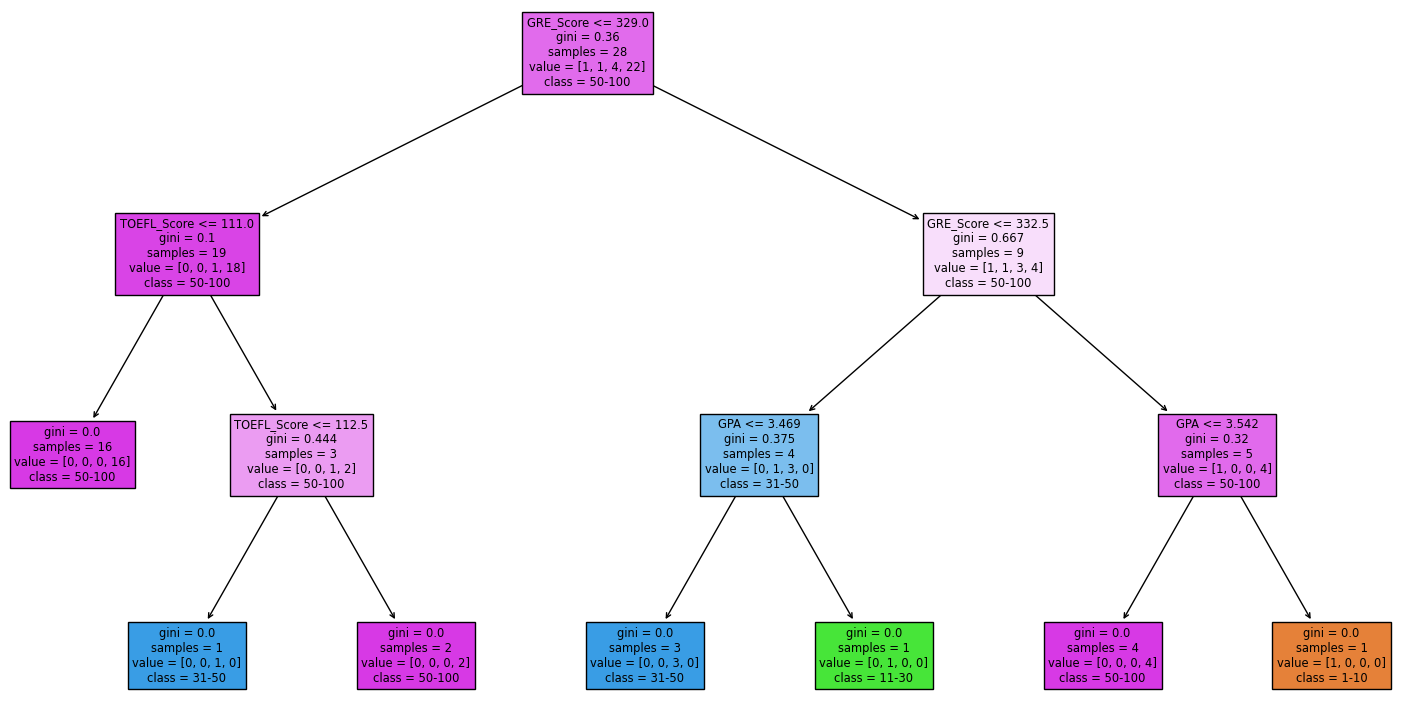
\includegraphics[width=\textwidth]{images/QS决策树.png}
    \caption{Decision Tree}
    \label{fig:my_label}
\end{figure}


\section{Conclusion and Self-Evaluation}

With the data stored in our database system with choreographed relational schema and our data mining approach, we believe that the designed system involves notable educational and commercial significance where we are able to provide our customer students with meaningful services. To finish the project, all group members have contributed greatly and equally.\\

From this project, we learned about designing a well-structured relational database for an educational organization, including identifying entities, relationships, and constraints. We encountered several problems, including how to determine normalization levels, how to set foreign key constraints and how to create ER diagram. Limitations include the potential for outdated or incomplete information, and the need to maintain referential integrity.

\section{References}
• Data from: https://opencs.app

\section{Appendices}
\noindent
1. Sample data: see excel files in folder "Data". We use python to insert those .xlsx files to the database. Insertion of data: inser data.py\\
2. SQL codes: creation of the database is in create.sql. Queries are in query.sql\\
3. PPT: EduSpark.pptx\\
4. Decision tree: decision tree.py\\
\end{spacing}

%\FloatBarrier

\end{document}
